%%%%%%%%%%%%%%%%%%%%%%%%%%%%%%%%%%%%%%%%%
% Jacobs Landscape Poster
% LaTeX Template
% Version 1.1 (14/06/14)
%
% Created by:
% Computational Physics and Biophysics Group, Jacobs University
% https://teamwork.jacobs-university.de:8443/confluence/display/CoPandBiG/LaTeX+Poster
%
% Further modified by:
% Nathaniel Johnston (nathaniel@njohnston.ca)
%
% This template has been downloaded from:
% http://www.LaTeXTemplates.com
%
% License:
% CC BY-NC-SA 3.0 (http://creativecommons.org/licenses/by-nc-sa/3.0/)
%
%%%%%%%%%%%%%%%%%%%%%%%%%%%%%%%%%%%%%%%%%

%----------------------------------------------------------------------------------------
%	PACKAGES AND OTHER DOCUMENT CONFIGURATIONS
%----------------------------------------------------------------------------------------

\documentclass[final]{beamer}

\usepackage[scale=1.1]{beamerposter} % Use the beamerposter package for laying out the poster
\usepackage[francais]{babel}
\usepackage[utf8]{inputenc}

\usetheme{confposter} % Use the confposter theme supplied with this template

\setbeamercolor{block title}{fg=ngreen,bg=white} % Colors of the block titles
\setbeamercolor{block body}{fg=black,bg=white} % Colors of the body of blocks
\setbeamercolor{block alerted title}{fg=white,bg=dblue!70} % Colors of the highlighted block titles
\setbeamercolor{block alerted body}{fg=black,bg=dblue!10} % Colors of the body of highlighted blocks
% Many more colors are available for use in beamerthemeconfposter.sty

%-----------------------------------------------------------
% Define the column widths and overall poster size
% To set effective sepwid, onecolwid and twocolwid values, first choose how many columns you want and how much separation you want between columns
% In this template, the separation width chosen is 0.024 of the paper width and a 4-column layout
% onecolwid should therefore be (1-(# of columns+1)*sepwid)/# of columns e.g. (1-(4+1)*0.024)/4 = 0.22
% Set twocolwid to be (2*onecolwid)+sepwid = 0.464
% Set threecolwid to be (3*onecolwid)+2*sepwid = 0.708

\newlength{\sepwid}
\newlength{\onecolwid}
\newlength{\twocolwid}
\newlength{\threecolwid}
\setlength{\paperwidth}{48in} % A0 width: 46.8in
\setlength{\paperheight}{36in} % A0 height: 33.1in
\setlength{\sepwid}{0.024\paperwidth} % Separation width (white space) between columns
\setlength{\onecolwid}{0.22\paperwidth} % Width of one column
\setlength{\twocolwid}{0.464\paperwidth} % Width of two columns
\setlength{\threecolwid}{0.708\paperwidth} % Width of three columns
\setlength{\topmargin}{-0.5in} % Reduce the top margin size
%-----------------------------------------------------------

\usepackage{graphicx}  % Required for including images

\usepackage{booktabs} % Top and bottom rules for tables

%----------------------------------------------------------------------------------------
%	TITLE SECTION
%----------------------------------------------------------------------------------------

\title{Calibration en finance : Mélange de modèles de \bsc{Black-Scholes}} % Poster title

\author{\bsc{Kheldouni} Mohammed-Amine
\\\vspace{1cm} Octobre 2016 - février 2017 \hspace{3cm} \textbf{ENPC}
\\\vspace{1cm} \textbf{Encadr\'e par :}
Bernard \bsc{Lapeyre}, Professeur à l'Ecole des Ponts ParisTech et Chercheur au CERMICS} % Author(s)

\institute{\vspace{-2cm}}

%----------------------------------------------------------------------------------------

\begin{document}

\addtobeamertemplate{block end}{}{\vspace*{2ex}} % White space under blocks
\addtobeamertemplate{block alerted end}{}{\vspace*{2ex}} % White space under highlighted (alert) blocks

\setlength{\belowcaptionskip}{2ex} % White space under figures
\setlength\belowdisplayshortskip{2ex} % White space under equations

\begin{frame}[t] % The whole poster is enclosed in one beamer frame

\begin{columns}[t] % The whole poster consists of three major columns, the second of which is split into two columns twice - the [t] option aligns each column's content to the top

\begin{column}{\sepwid}\end{column} % Empty spacer column

\begin{column}{\onecolwid} % The first column

%----------------------------------------------------------------------------------------
%	OBJECTIVES
%----------------------------------------------------------------------------------------

\begin{alertblock}{Objectifs}
\begin{itemize}
  \item Comprendre comment évaluer le prix d'un sous-jacent avec une modélisation mathématique du marché.
  \item Confronter le modèle à ses limites en terme de calibration financière.
  \item Appliquer des notions stochastiques à la finance et connaître l'utilité de tels modèles.
\end{itemize}

\end{alertblock}


%----------------------------------------------------------------------------------------
%	INTRODUCTION
%----------------------------------------------------------------------------------------
\vspace{2cm}
\begin{block}{Notions financières}
  \begin{itemize}
    \item une option est un produit dérivé qui établit un contrat entre un acheteur et un vendeur.
    \item $T$ est la maturité ou l'échéance. C'est la date à laquelle une opération doit être réalisée.
    \item $S_t$ : L'actif sous-jacent à l'instant t est l'actif sur lequel porte une option.
    \item $r$ : Le taux d'intérêt.
    \item $\sigma$ : La volatilité, elle indique l'ampleur des variations du cours d'un actif financier.
    \item $K$ : Le strike désigne le prix d'exercice d'une option, qui correspond au prix fixé dans le contrat pour l’acquisition ou la cession du sous-jacent.
    \item \textit{Call} : Option d'achat d'un instrument financier.
    \item \textit{Put} : Option de vente de cet instrument.
  \end{itemize}
  \vspace{2cm}
  \begin{alertblock}{Mise en situation}
    Etant donné les paramètres $\sigma$, $T$, $K$, $S_0$ et $r$ on voudrait calculer le prix d'un call ou d'un put sur le marché, pour un actif financier.
    \newline
    Pour cela, on admet le modèle de \bsc{Black-Scholes}, qui donne sous certaines hypothèses le pix d'un \textit{Call} ou d'un \textit{Put}. Ce modèle est démontré dans le livre de Philippe  \bsc{BRIAND} sur le modèle de \bsc{Black-Scholes}.
    \newline
  \end{alertblock}
\end{block}

%----------------------------------------------------------------------------------------


%----------------------------------------------------------------------------------------

\end{column} % End of the first column

\begin{column}{\sepwid}\end{column} % Empty spacer column

\begin{column}{\twocolwid} % Begin a column which is two columns wide (column 2)
\vspace{-1cm}
\begin{block}{Modèles de \bsc{Black-Scholes} et problèmes de calibration}

\begin{columns}[t,totalwidth=\twocolwid] % Split up the two columns wide column

\begin{column}{\onecolwid} % The first column within column 2 (column 2.1)

%----------------------------------------------------------------------------------------
%	MATERIALS

\begin{alertblock}{Modèle de \bsc{Black-Scholes}}
  Dans ce modèle, on considère le prix de l'action comme un processus stochastique en temps continu $S_t$ et suit certaines hypothèses. \newline
  {\center{\textbf{Equation différentielle stochastique}}
  \[ {\color{red} dS_t = \mu S_t dt + \sigma S_t dW_t} \]}
avec $W_t$ Un mouvement Brownien standard.
\newline
Le prix d'un \textit{Call} est caractérisé par son \textit{payoff} $(S_T - K)_{+}$. \newline
Le modèle fournit la formule de \bsc{Black-Scholes} d'un \textit{Call} (resp. d'un \textit{Put}) :
$$ C(S_0,K,r,t,\sigma) = S_0 \phi(d_1)-K \times e^{-rt} \phi(d_2) $$
$$ P(S_0,K,r,t,\sigma) = -S_0 \phi(-d_1)+K \times e^{-rt} \phi(-d_2) $$
Avec : \begin{itemize}
\item $\phi$ la fonction de répartition de la loi normale centrée réduite.
\item $d_1 = \frac{1}{\sigma \sqrt{t}} (ln(\frac{S_0}{K})+(r+\frac{1}{2}\sigma^2)t) $
\item $d_2 = d_1 - \sigma \sqrt{t}$
\end{itemize}
\end{alertblock}
On fixe un nombre $P$ de modèles de Black-Scholes dont on va effectuer un mélange selon une certaine distribution de probabilités $(p_1,p_2,...,p_p)$.
\newline
Ainsi on considère le \texit{Call}, à $K$, $r$ et $t$ fixés, de notre mélange comme suit :
$$ C_m(\lambda, \sigma, p) = \sum^p_{i=1} p_i C(\lambda_i,K,r,t,\sigma_i) $$
\vspace{-0.3cm}
$\lambda = (S_{0,1},...,S_{0,P}),\ \  \sigma = (\sigma_1,...,\sigma_P), \ \ p = (p_1,...,p_P)$
%----------------------------------------------------------------------------------------

\end{column} % End of column 2.1

\begin{column}{\onecolwid} % The second column within column 2 (column 2.2)

%----------------------------------------------------------------------------------------
%	METHODS
%----------------------------------------------------------------------------------------
\begin{figure}[!H]
  \centerline{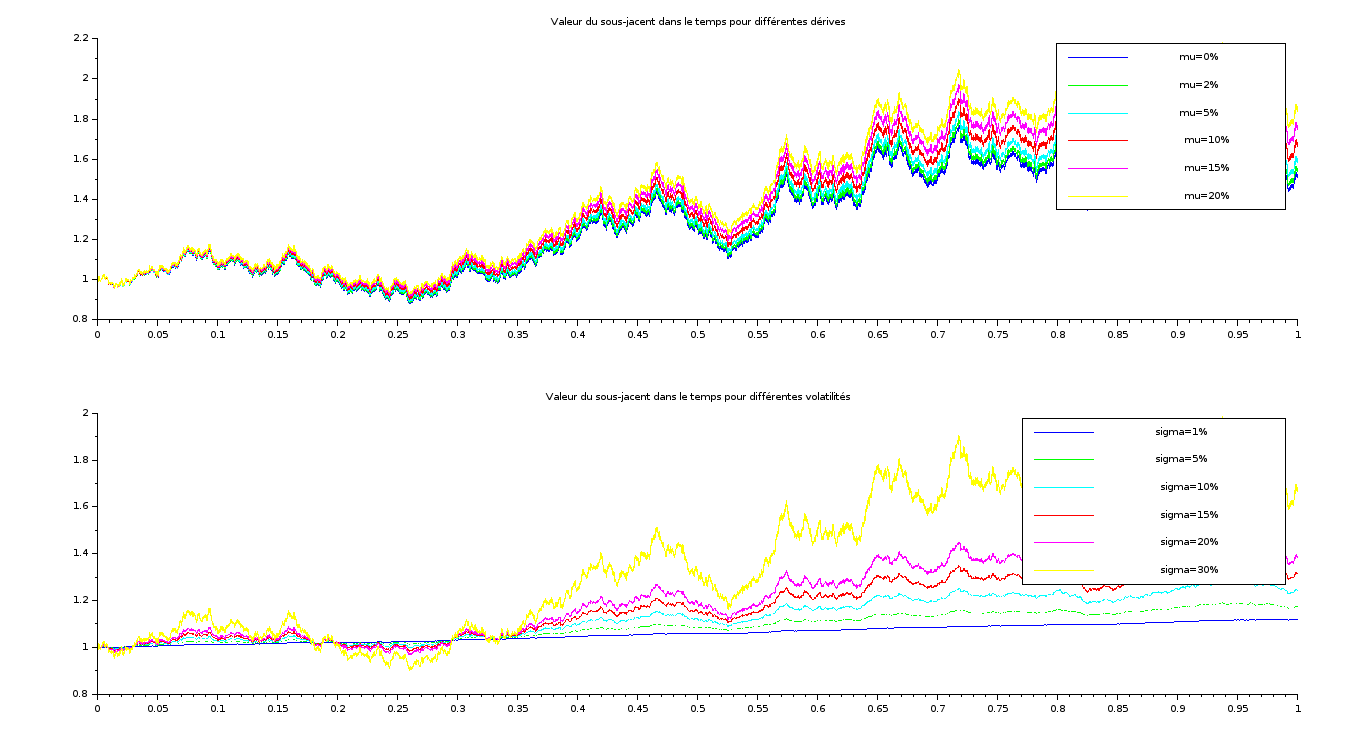
\includegraphics[scale=0.65]{bs_actif_mopsi.png}}

\end{figure}

\vspace{0.3cm}
\begin{alertblock}{Calibration en finance}
  $ \beta_* = (\lambda,\sigma,p)$ sont nos données de départ pour $K$ fixé.
  \newline
  On retrouve la valeur $\beta_*$ par une méthode des moindres carrés sur plusieurs prix d'exercice $(K_1,...,K_M)$, minimisant les résidus des prix. \newline
  Pour un call :
  \[{\color{red} \min \sum^M_{j=1} (C_{m,j}(\beta)-\alpha_j)^2} \]
  \vspace{-0.4cm}
  \[ s.c. {\color{red} \sum^p_{i=1}p_i = 1} \]
$\alpha_j$ étant le prix du Call calculé avec les valeurs de $\beta_*$ pour un \textit{Strike} $K_j$.
\newline
Il est important de comprendre que cette méthode d'optimisation prouve une certaine bijection entre les valeurs financières $\lambda$, $\sigma$ et la distribution $p$ du mélange et le prix d'une option (d'achat ou de vente) sur le marché.
\end{alertblock}
\end{column} % End of column 2.2
%----------------------------------------------------------------------------------------

\end{columns} % End of the split of column 2 - any content after this will now take up 2 columns width

\end{block}


%----------------------------------------------------------------------------------------
\vspace{0cm}
\begin{block}{Résultats}

\setbeamercolor{block title}{fg=ngreen,bg=dblue!10} % Colors of the block titles
\setbeamercolor{block body}{fg=black,bg=dblue!10} % Colors of the body of blocks

\begin{columns}[t,totalwidth=0.45\paperwidth] % Split up the two columns wide column again

\begin{column}{\onecolwid} % The first column within column 2 (column 2.1)

%----------------------------------------------------------------------------------------
%	MATHEMATICAL SECTION
%----------------------------------------------------------------------------------------

\begin{minipage}{0.49\textwidth}
  \vspace{2cm}
  On prend $P = 2$
  \begin{itemize}
    \item $\lambda = (100,100)$
    \item $\sigma = (0.2, 0.4)$
    \item $p = (0.5,0.5) $
    \item $r = 0$
    \item $K = (50,...150)$
  \end{itemize}
\end{minipage}

\begin{minipage}{1.49\textwidth}
\begin{figure}[!r]
  \vspace{-10cm}
  \hspace{-4cm}
  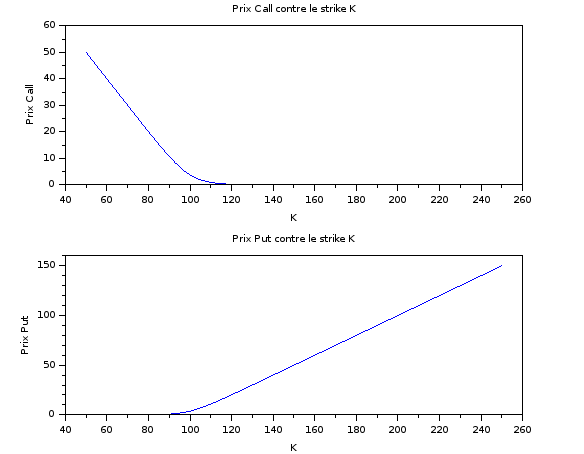
\includegraphics[scale=0.8]{callput.png}
\end{figure}
\end{minipage}
\newline
\newline
\\
  On trouve par la fonction d'optimisation non linéaire de SCILAB, \textit{optim}, un $\beta$ proche de l'optimum avec une erreur assez faible :
%----------------------------------------------------------------------------------------

\end{column} % End of column 2.1

\begin{column}{\onecolwid} % The second column within column 2 (column 2.2)

%----------------------------------------------------------------------------------------
%	RESULTS
%----------------------------------------------------------------------------------------


  $$ \beta_{approx} = (100.001,100.001,0.22,0.36,0.5,0.5) $$
  $$ \Rightarrow \ \ \ \ \epsilon = \frac{\|\beta_{approx}-\beta_* \|}{\|\beta_* \|} \approx 3.16 \times 10^{-4}$$
  \textbf{Les problèmes de calibration :}
  \begin{itemize}
    \item L'ensemble des solutions réalisables est trop grand.
    \item Choix d'un bon intervalle d'exercice $K$.
    \item En dimension plus grande, les erreurs de calibration sont encore plus importantes.
  \end{itemize}
    \center{\color{red}{\textbf{Les algorithmes d'optimisation rendent la procédure de calibration numériquement délicate en grande dimension P}}}
%----------------------------------------------------------------------------------------

\end{column} % End of column 2.2

\end{columns} % End of the split of column 2

\end{block}

\end{column} % End of the second column

\begin{column}{\sepwid}\end{column} % Empty spacer column

\setbeamercolor{block title}{fg=ngreen,bg=white} % Colors of the block titles
\setbeamercolor{block body}{fg=black,bg=white} % Colors of the body of blocks

\begin{column}{\onecolwid} % The third column

%----------------------------------------------------------------------------------------
%	CONCLUSION
%----------------------------------------------------------------------------------------

\begin{block}{Volatilité implicite}
On souhaite parfois retrouver la volatilité à travers le modèle de \bsc{Black-Scholes} pour anticiper sur le prix d'un actif. \newline
Comme démontré dans le livre de Peter \bsc{TANKOV}, l'inversion de la formule de \bsc{Black-Scholes} est possible :
  $$ \exists ! \sigma_* / \ \ \ C_{BS}(S_0,K,r,t,\sigma_*) = C_{marché} $$
  On appelle cette volatilité, la \textbf{volatilité implicite}.
\newline
  En utilisant un algorithme de dichotomie ou une méthode de Newton sur \bsc{SCILAB}, on obtient un graphe tridimensionnel appelé \textbf{la surface de la volatilité}.
    \begin{figure}
      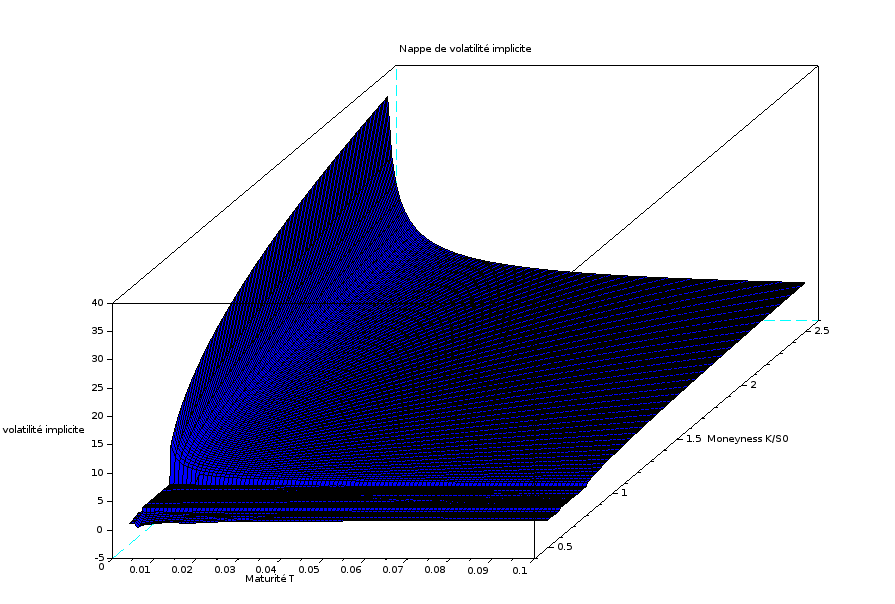
\includegraphics[scale=0.80]{volimpl1.png}
      \label{Exemple de surface de volatilité}
    \end{figure}
\end{block}

\begin{block}{Application à un actif :}
  \begin{minipage}{0.49\textwidth}
    On prend $M = 200$ et :
      \[
        \begin{array}{|c|c|}
          \hline
          S_0 & \$ 505.15  \\ \hline
          \sigma_0 & 20\% \\ \hline
          r & 3.3 \% \\ \hline
          K & (\$500,...,\$700) \\ \hline
          T & 2 \;mois \\ \hline
        \end{array}
      \]
  \end{minipage}

  \begin{minipage}{1.49\textwidth}
    \begin{figure}
      \vspace{-8.5cm}
      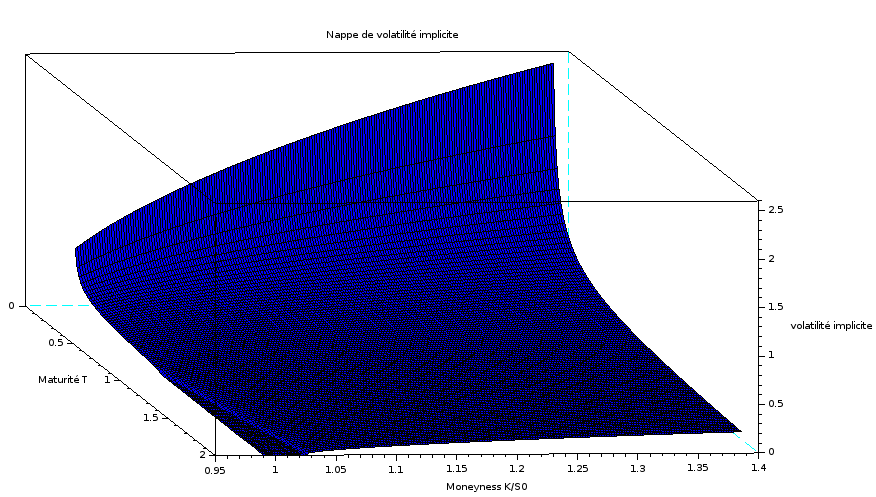
\includegraphics[scale=0.55]{volimpl2.png}
    \end{figure}
  \end{minipage}
\end{block}

%----------------------------------------------------------------------------------------
%	ADDITIONAL INFORMATION
%----------------------------------------------------------------------------------------

%----------------------------------------------------------------------------------------
%	REFERENCES
%----------------------------------------------------------------------------------------

\begin{block}{Références}

  \begin{minipage}{0.6\textwidth}
    \begin{itemize}
      \small
        \item Philippe \bsc{BRIAND},  \textit{Le modèle de Black-Scholes}, 2003.
        \item Peter \bsc{TANKOV}, \textit{Surface de volatilité}, 2015.
        \item Damiano \bsc{BRIGO}, Fabio \bsc{MERCURIO}, \textit{Lognormal-mixture dynamics and calibration to market volatility smiles}.
        \item Pr. Benoite \bsc{DE-SAPORTA}, \textit{TP sur les mouvements Brownien et Modèle de \bsc{Black-Scholes} (finance en temps continu)}
    \end{itemize}
    \end{minipage}

    \begin{minipage}{1.49\textwidth}

  \begin{center}

      \vspace{-6cm}
      \hspace{3cm}
      
\includegraphics[scale=0.2]{logos.png}
  \end{center}
    \end{minipage}
\end{block}
%\begin{frame}{Bibliographie}
%\begin{itemize}

%   \item \url{https://fr.wikipedia.org/wiki/Maturit%C3%A9_(finance)}
%   \item \url{https://fr.wikipedia.org/wiki/Action_(finance)}
%   \item \url{https://fr.wikipedia.org/wiki/Actif_sous-jacent}
%   \item \url{https://fr.wikipedia.org/wiki/Taux_d%27int%C3%A9r%C3%AAt}
%   \item \url{https://fr.wikipedia.org/wiki/Volatilit%C3%A9_(finance)}
%\end{itemize}
%\end{frame}

%----------------------------------------------------------------------------------------

\end{column} % End of the third column

\end{columns} % End of all the columns in the poster

\end{frame} % End of the enclosing frame

\end{document}
